\subsection{Batch}\label{Batch}

Batch processing is one of the earliest processes. As name suggests, in batch processing we are expecting multiple files (batch) \parencite{web:Amazon}. Once they are received, they are being processed.

One real world example is roller coaster. In order to operate the ride in optimal capacity, we need 20 (an example number) people on it. The idea is for operator to fill the ride with 20 people. After the ride is complete, the next 20 are selected.

Similar process is in batch processing. Computer (server) waits for n number of files. After they are received, they are inserted into data pipeline in order to start the operation. Limits can be set if files are not received (but this could then be considered hybrid processing).

In our case, we are using batch processing with flamingo data. Files are downloaded from the web and once they are ready pipeline is triggered.


\begin{figure}[H]
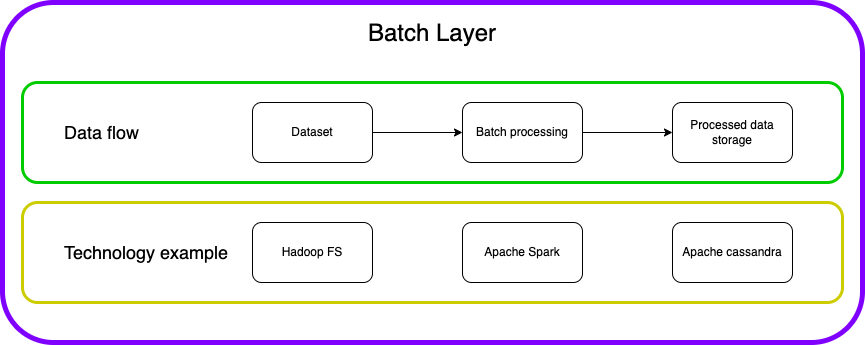
\includegraphics[scale=0.45]{img/ProcessingParadigms/BigData-Batch.png}
\centering
\caption{Batch}
\label{fig:Batch}
\end{figure}